\documentclass[tikz, border=2pt]{standalone}
% main document, called main.tex
\usepackage{tikz}

\begin{document}

\usetikzlibrary{decorations.pathreplacing}

    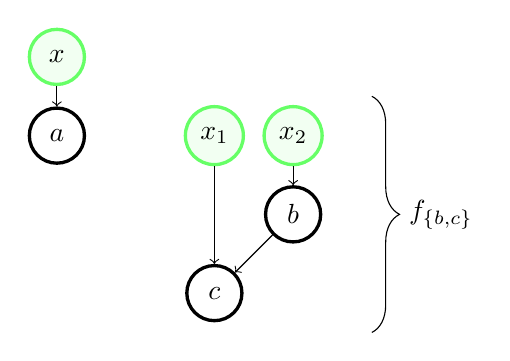
\begin{tikzpicture}[
        scale=1.0,
        inv/.style={circle, draw=green!60, fill=green!5, very thick, minimum size=7mm},
        opv/.style={circle, draw=black, very thick, minimum size=7mm},
      ]
      \node[inv] (x) at (-2,3)  {$x$};
      \node[opv] (a) at (-2,2)  {$a$};

      \node[inv] (x1) at (0,2)  {$x_1$};
      \node[inv] (x2) at (1,2)  {$x_2$};
      \node[opv] (b) at (1,1)  {$b$};
      \node[opv] (c) at (0,0)  {$c$};

      \draw (x) edge[->] (a)
            (x1) edge[->] (c)
            (x2) edge[->] (b)
            (b) edge[->] (c);

      %% \draw[
      %%   decorate,decoration={brace,amplitude=10pt}
      %% ] (-3,1.5) -- (-3,3.5) node[black,midway,xshift=-20pt] {$h$};
      \draw[
        decorate,decoration={brace,amplitude=10pt,mirror}
      ] (2,-.5) -- (2,2.5) node[black,midway,xshift=25pt] {$f_{\{b,c\}}$};
    \end{tikzpicture}

\end{document}
